\part{Elektrotechnik}
	\section{Grundlagen}
		\subsection{Maxwell-Gleichungen}
			\subsubsection{Mikroskopisch}
				Die mikroskopischen Maxwell-Gleichungen verknüpfen die elektrische Feldstärke $ \bm{E} $ und die magnetische Flussdichte $ \bm{B} $ mit der Ladungsdichte $ \bm{\rho} $  (Ladung pro Volumen) und der elektrischen Stromdichte $ \bm{S} $ (Strom pro durchflossene Fläche).
				\begin{enumerate}
					\item \textbf{Maxwell'sche Gleichung - Durchflutungsgesetz}
						 \begin{equation}
						 \boxed{\text{rot} (\bm{B}) = \mu_{0}\bm{S} +  \mu_{0}\varepsilon_{0}\frac{\partial\bm{E}}{\partial t}}
						 \end{equation}
						 
					\item \textbf{Maxwell'sche Gleichung - Induktionsgesetz}
					
	
					\item \textbf{Maxwell'sche Gleichung - Gauß'sches Gesetz}
					
					\item \textbf{Maxwell'sche Gleichung - Gauß'sches Gesetz für Magnetfelder}
				\end{enumerate}
			\subsubsection{Makroskopisch}
				Bei Anwesenheit von Materie sind die mikroskopischen Maxwell-Gleichungen einerseits unhandlich, da schließlich jeder Ladungsträger in jedem Atom des Mediums berücksichtigt werden muss. Andererseits können die magnetischen Eigenschaften (beispielsweise von einem Permanentmagneten) prinzipiell nicht ohne zusätzliche physikalische Erkenntnisse der Quantenmechanik aus den mikroskopischen Maxwell-Gleichungen abgeleitet werden. Die makroskopischen Maxwell-Gleichungen berücksichtigen die Eigenschaften der Materie in Form von Materialparametern, wobei dem leeren Raum die Parameter Permittivität $ \varepsilon_{0} $ und Permeabilität $ \mu_{0} $ zugeordnet werden. \\
				Die Anwesenheit von Materie erfordert, dass das elektrische und das magnetische Feld jeweils durch zwei zusätzliche Vektorfelder beschrieben werden, der elektrischen Flussdichte $ \bm{D} := \varepsilon_{0}\bm{E} + \bm{P} $ und der magnetischen Feldstärke $ \bm{H} := \frac{1}{\mu_{0}}\bm{B} - \bm{M} $. Dabei wird $ \bm{P} $ als Polarisation und $ \bm{M} $ als Magnetisierung bezeichnet.
				\begin{enumerate}
					\item \textbf{Maxwell'sche Gleichung - Durchflutungsgesetz}
					\begin{equation}
						\nabla \bm{\times} \bm{H} = \text{rot} (\bm{H}) = \bm{S} +  \frac{d\bm{D}}{dt}  \quad	\text{bzw.}	 \quad \oint_{S} \bm{H}\cdot d\bm{s} = \int_{A}\bigg(\bm{S} + \frac{d\bm{D}}{dt}\bigg) d\bm{A}
					\end{equation}	
					Die 1. Maxwellgleichung besagt, dass das Umlaufintegral der magnetischen Feldstärke $ \bm{H} $ gleich dem umschlossenen Strom ist. Dabei spielt es keine Rolle ob der Strom an Ladungsträger gebunden ist oder als Verschiebestrom vorhanden ist. Man kann auch sagen, dass elektrische Ströme, einschließlich Verschiebeströme, zu einem magnetischen Wirbelfeld führen.
					
					\item \textbf{Maxwell'sche Gleichung - Induktionsgesetz}
					\begin{equation}
						\bm{\nabla} \times \bm{E} = \text{rot} (\bm{E}) = -\frac{\partial \bm{B}}{\partial t}\quad 	\text{bzw.}	 \quad \oint_{S} \bm{E}\cdot  d\bm{s} = -\frac{d}{dt} \int_{A} \bm{B}\cdot d\bm{A}
					\end{equation}
					
					\item \textbf{Maxwell'sche Gleichung - Quellenfreiheit (Divergenzfreiheit) des magnetishen Feldes}
					\begin{equation}
						\bm{\nabla} \cdot \bm{B}= \text{div}(\bm{B}) = 0
					\end{equation}
					
					\item \textbf{Maxwell'sche Gleichung - Quellenbehaftetes elektrisches Feldes (Divergenz)}
					\begin{equation}
						\bm{\nabla}\cdot \bm{D} = \text{div}(\bm{D}) = \rho
					\end{equation}
				\end{enumerate}
		
		
		\subsection{\textcolor{red}{Dielektrizität - Permittivität}}
		\subsection{Reluktanzkraft/ Maxwellkraft-Prinzip} \label{reluktanzkraft}
		Bei einer stromdurchflossenen Spule, die wie in der Abbildung um einen Eisenkern gewickelt ist, erzeugt die Spule einen magnetischen Fluss im Eisenkern. Es entstehen in beiden Luftspaleten Anziehungskräfte auf den losen Eisenkörper (Anker). Der Effekt der Anziehung beruht darauf, dass die \textit{Reluktanz}, also der magnetishe Widerstand, reduziert und die Induktivität erhöht wird. Das ist der Fall wenn die Feldlinien durch den Anker verlaufen. Wird der Abstand zwischen dem Anker und den Magnetpolen verkürzt, verringert sich der magnetische Widerstand der Feldlinien, denn der Widerstand ist im Eisen wesentlich kleiner als in der Luft.
		\begin{figure}[h]
			\centering
			\includegraphics[width=0.2\linewidth]{./pics/reluktanz}
		\end{figure}
		
		
		\subsection{Magnetische Permeabilität}
			Auch magnetische Leitfähigkeit genannt. Sie dient als Faktor für die Abschwächung/ Verstärkung der magnetischen Flussdichte durch ein Material und ergibt sich als
			\[ \mu = \dfrac{B}{H} \]
			\leavevmode
			\tab[1cm] \textbf{B} \tab ... \tab magnetische Flussdichte [$ \frac{Vs}{m^{2}} $]\\
			\tab[1cm] \textbf{H} \tab ... \tab magnetische Feldstärke [$ \frac{A}{m} $]\\\\
			Die magnetische Permeabilität wird dabei durch eine Naturkonstante skaliert, die sogenannte magnetische Feldkonstante $ \mu_{0} = 4\pi\cdot 10^{-7} Vs/Am $. Sie gibt die magnetische Leitfähigkeit des Vakuums an. Für jedes Material kann die magnetische Permeabilität als Produkt aus der Permeabilitätszahl und der magnetischen Feldkonstante angegeben werden.
			\[ \mu = \mu_{r}\cdot\mu_{0}\]
			\tab[1cm] \textbf{$ \bm{\mu_{r}} $} \tab ... \tab relative magnetische Permeabilität (auch Permeabilitätszahl) [dimensionslos]\\\\
			Die Materialkonstante ist für Paramagnetika $ \mu_{r} > 1 $, Diamagnetika $ \mu_{r} = 1$ und für Ferro-, Ferri und Antiferromagnetika eine komplizierte Funktion von Feldstärke und Vorgeschichte ($ \mu_{r} $ bis $ 10^{5} $).\\\\
			\textbf{Diamagnetika:} Gold, $ CO_{2} $, Kupfer, Wasser, Zink, ... \\
			\textbf{Paramagnetika:} Mangan, Chrom, Natrium, Aluminium, ... Auch alle Ferromagnetika gehören dazu. Bei Stoffen in denen Dipole durch ein äußeres Magnetfeld ausgerichtet werden können und dieses somit verstärken.\\
			\textbf{Ferromagnetika:} Eisen, Cobalt, Nickel, ... \\
			\textbf{Ferrimagnetismus:} Kristallstruktur innerhalb welcher sich die magnetischen Momente der Atome abwechselnd antiparallel ausrichten. Diese heben sich gegenseitig aber nicht wie beim Antiferromagnetismus vollständig auf, sondern eine der beiden Richtungen ist stärker.
			
	
		\subsection{Wirbelströme}
			Wie im Induktionsgesetz beschrieben, wird in einem elektrischer Leiter ein Strom induziert wenn sich dieser in einem konstanten Magnetfeld bewegt oder sich in Ruhe in einem sich wechselnden Magnetfeld befindet (= magnetische Flussänderung). Bei einem Draht ist die Stromrichtung eindeutig vorgegeben. Handelt es sich jedoch um einen Leiter mit großer Oberfläche, dann bilden die induzierten Ströme sogenannte Ringströme/Wirbelströme. 
			\begin{figure}[h]
				\centering
				\includegraphics[width=0.7\linewidth]{./pics/Wirbel2.jpg}
				\caption{Induktion eines Wirbelstromes}
			\end{figure}
			\leavevmode \\
			Dies ist beispielsweise bei Transformatoren oder Generatoren der Fall. Da Wirbelströme zu Energieverlusten führen, müssen diese durch etwa die Verwendung von Blechpaketen statt einem dicken Eisenkern, reduziert werden. Dabei sind einzelne Bleche elektrisch voneinander isoliert.
			
	\section{\textcolor{red}{Filter}}
		\subsection{Filtertypen}
		\begin{itemize}
			\item Tiefpassfilter
			\item Hochpassfilter
			\item Bandpassfilter
			\item Bandsperre, Kerbfilter
			\item Allpassfilter – lässt alle Frequenzen mit gleicher Verstärkung durch, kann aber eine Phasenverschiebung verursachen.
		\end{itemize}
		Die Filterordnung beschreibt die Dämpfung von Frequenzen unterhalb od. oberhalb der Grenzfrequenz. Z.b. bei einem Filter n. Ordnung würde die TF mit $ n\cdot6dB/Oktave $ fallen.\\\\
		Weitere Einteilungen: Aktiv, Passiv, Linear, Nicht-Linear, Ordnung
		\subsection{\textcolor{red}{Analoges aktives Filter}}
		\subsection{\textcolor{red}{Analoges passives Filter}}
			\subsubsection{\textcolor{red}{Topologien}}
			https://de.wikipedia.org/wiki/Analogfilter\\
			http://elektroniktutor.de/analogtechnik/filter.html
			\subsubsection{\textcolor{red}{Tiefpassfilter}}
				Praktische Anwendung, wie wird ein Tiefpassfilter dimensioniert --> gewünschte Grenzfrequenz einstellen
			\subsubsection{\textcolor{red}{Hochpassfilter}}
			\subsubsection{Notchfilter}
				Ein Kerbfilter ist ein elektronisches Filter, mit dem Frequenzen innerhalb eines engen Frequenzbereiches ausgefiltert werden können. Anschaulich wird eine Kerbe in das Frequenzdiagramm eingefügt.
				Kerbfilter stellen einen besonders schmalbandigen Typ von Bandsperrfilter dar, welche in der Übertragungsfunktion nur eine Nullstelle aufweisen und damit nicht ein breites Frequenzband, sondern idealerweise genau eine Frequenz möglichst stark dämpfen.
				
		\subsection{\textcolor{red}{Digitales Filter}}
			\subsubsection{\textcolor{red}{FIR - Finite Impulse Response}}
			\subsubsection{\textcolor{red}{IIR - Infinite Impulse Response}	}		
		\subsection{Kalmanfilter}
			Ein Kalman-Filter schätzt den Wert einer ungenauen oder unsicheren Messung anhand der vorhergegangen Messwerte ab. Das Prinzip beruht auf Wahrscheinlichkeitsfunktionen. Systemzustände müssen dafür bekannt sein und fließen in die Berechnung mit ein. Anders formuliert wird eine Vorhersage des nächsten Wertes anhand des momentanen Wertes und der bekannten System-Eingangsvariablen geschätzt. Zusätzlich vergrößern die nicht abschätzbaren Parameter den Wahrscheinlichkeitsbereich, wo der nächste Wert landen könnte. Hinzu kommt nun noch eine Wahrscheinlichkeit für den Messwert des Sensors. Aufgrund von Rauschen erhalten wir einen anderen Wert als real vorhanden ist. Diese Abweichung wird wiederum als Wahrscheinlichkeit beschrieben. Nun kann man die beiden Wahrscheinlichkeiten (die des nächsten Wertes und der Korrektheit des Messwertes) multiplizieren und erhält einen neuen verbesserten Schätzwert.\\
			Dieser verbesserte Schätzwert kann nun wieder durch den ganzen Ablauf verwendet werden und wir erhalten einen neuen Schätzwert. Dieser Vorgang kann beliebig oft vorgenommen werden.
			Die Filter sind sehr schnell – Echtzeitfähig – und liefern in der Praxis sehr gute Ergebnisse. Zeigt sehr gute Filtereigenschaften für Sensorrauschen (Unsicherheit der Messung ausgleichen).\\
			http://www.bzarg.com/p/how-a-kalman-filter-works-in-pictures/
			
	\section{\textcolor{red}{Sensoren}}
		\subsection{\textcolor{red}{Übersicht von Sensoren nach deren Messgrößen}}
		Abstands- bzw. Wegsensoren
		Geschwindigkeits und Drehzahlsensoren
		Beschleunigungssensoren
		\subsection{\textcolor{red}{Piezoelektrische Sensoren}}
		\subsection{\textcolor{red}{Induktive Sensoren}}
		\subsection{\textcolor{red}{Kapazitive Sensoren}}
		\subsection{\textcolor{red}{Mechanische Sensoren}}
		\subsection{\textcolor{red}{Thermoelektrische Sensoren}}
		\subsection{\textcolor{red}{Resistive Sensoren}}
		\subsection{\textcolor{red}{Magnetische Sensoren}}
		\subsection{\textcolor{red}{Optische Sensoren}}
			\subsubsection{Interferometer}
				Das Messprinzip basiert auf der Überlagerung von zwei Wellen die unterschiedliche Wege zurücklegen. Grundsätzlich lässt sich mit jeder Art von Welle, seien es elektromagnetische Wellen, Schall- oder Materiewellen, eine Interferenz erzeugen.\\ Laserlicht eignet sich ausgezeichnet für kürzere (Meterbereich) und äußerst präzise (Pikometerbereich) Wegmessungen. Voraussetzung für eine erfolgreiche Interferenz ist, dass Wellen kohärent überlagert werden. Deshalb wird Laserlicht verwendet, da ausgesendete Lichtwellen nahezu phasengleich zueinander sind und eine sehr große Kohärenzlänge (max. Weglänge zweier Lichtstrahlen, bei der diese noch ein stabiles Interferenzmuster ergeben) - d.h. auch über große Distanzen phasengleich bleiben - besitzen. \\
				Die unterschiedlichen Typen von Interferometern haben meist das selbe Funktionsprinzip. Durch Überlagerung zweier Wellen, die in getrennten optischen Bahnen geführt und von Spiegeln bzw. einem Objekt reflektiert werden, bilden ein Interferenzmuster (Interferenzstreifen oder -ringe). Dieses ist abhängig von der Distanz des Objektes. Somit können Distanzänderungen detektiert werden.\\
				So werden beim \textbf{Michelson-Interferometer} durch einen Photosensor abwechselnd Minima und Maxima des Interferenzbildes registriert und mitgezählt. Wird die Anzahl der gemessenen Maxima mit der Wellenlänge des Laserlichts multipliziert, erhält man die Wegdifferenz. Da das Medium durch das die elektromagnetische Welle wandert, deren Wellenlänge beeinflusst, ist ein wichtiger Faktor, die Eigenschaften dieses Mediums zu berücksichtigen (Luftdruck, Luftfeuchtigkeit, Temperatur).\\
				Bei Vielstrahlinterferometern wie dem \textbf{Fabry-Per\'{o}t-Interferometer} wird die Längenänderung gemessen indem die Länge des optischen Resonators verändert wird. D.h. ein optischer Ausgang/Messkopf des Interferometers und das Objekt bilden gemeinsam einen optischen Resonator. Martin Zech von Attocube hat ein solches Interferometer entwickelt, das Genauigkeiten im sub-Nanometerbereich bei Raumtemperatur erreicht. Wird der Sensor mit flüssigem Helium auf 4 K gekühlt kann durch Rauschunterdrückung eine Genauigkeit von 1 pm erreicht werden.\\
		
				Vorteil:
				\begin{itemize}
					\item Höhere Empfindlichkeit 
					\item Längenmessungen bis 10$ ^{-12} $ m Genauigkeit können gemessen werden
				\end{itemize}
		
		
		

	\section{Elektrische Maschinen}
		\leavevmode
		\begin{figure}[h]
			\centering
			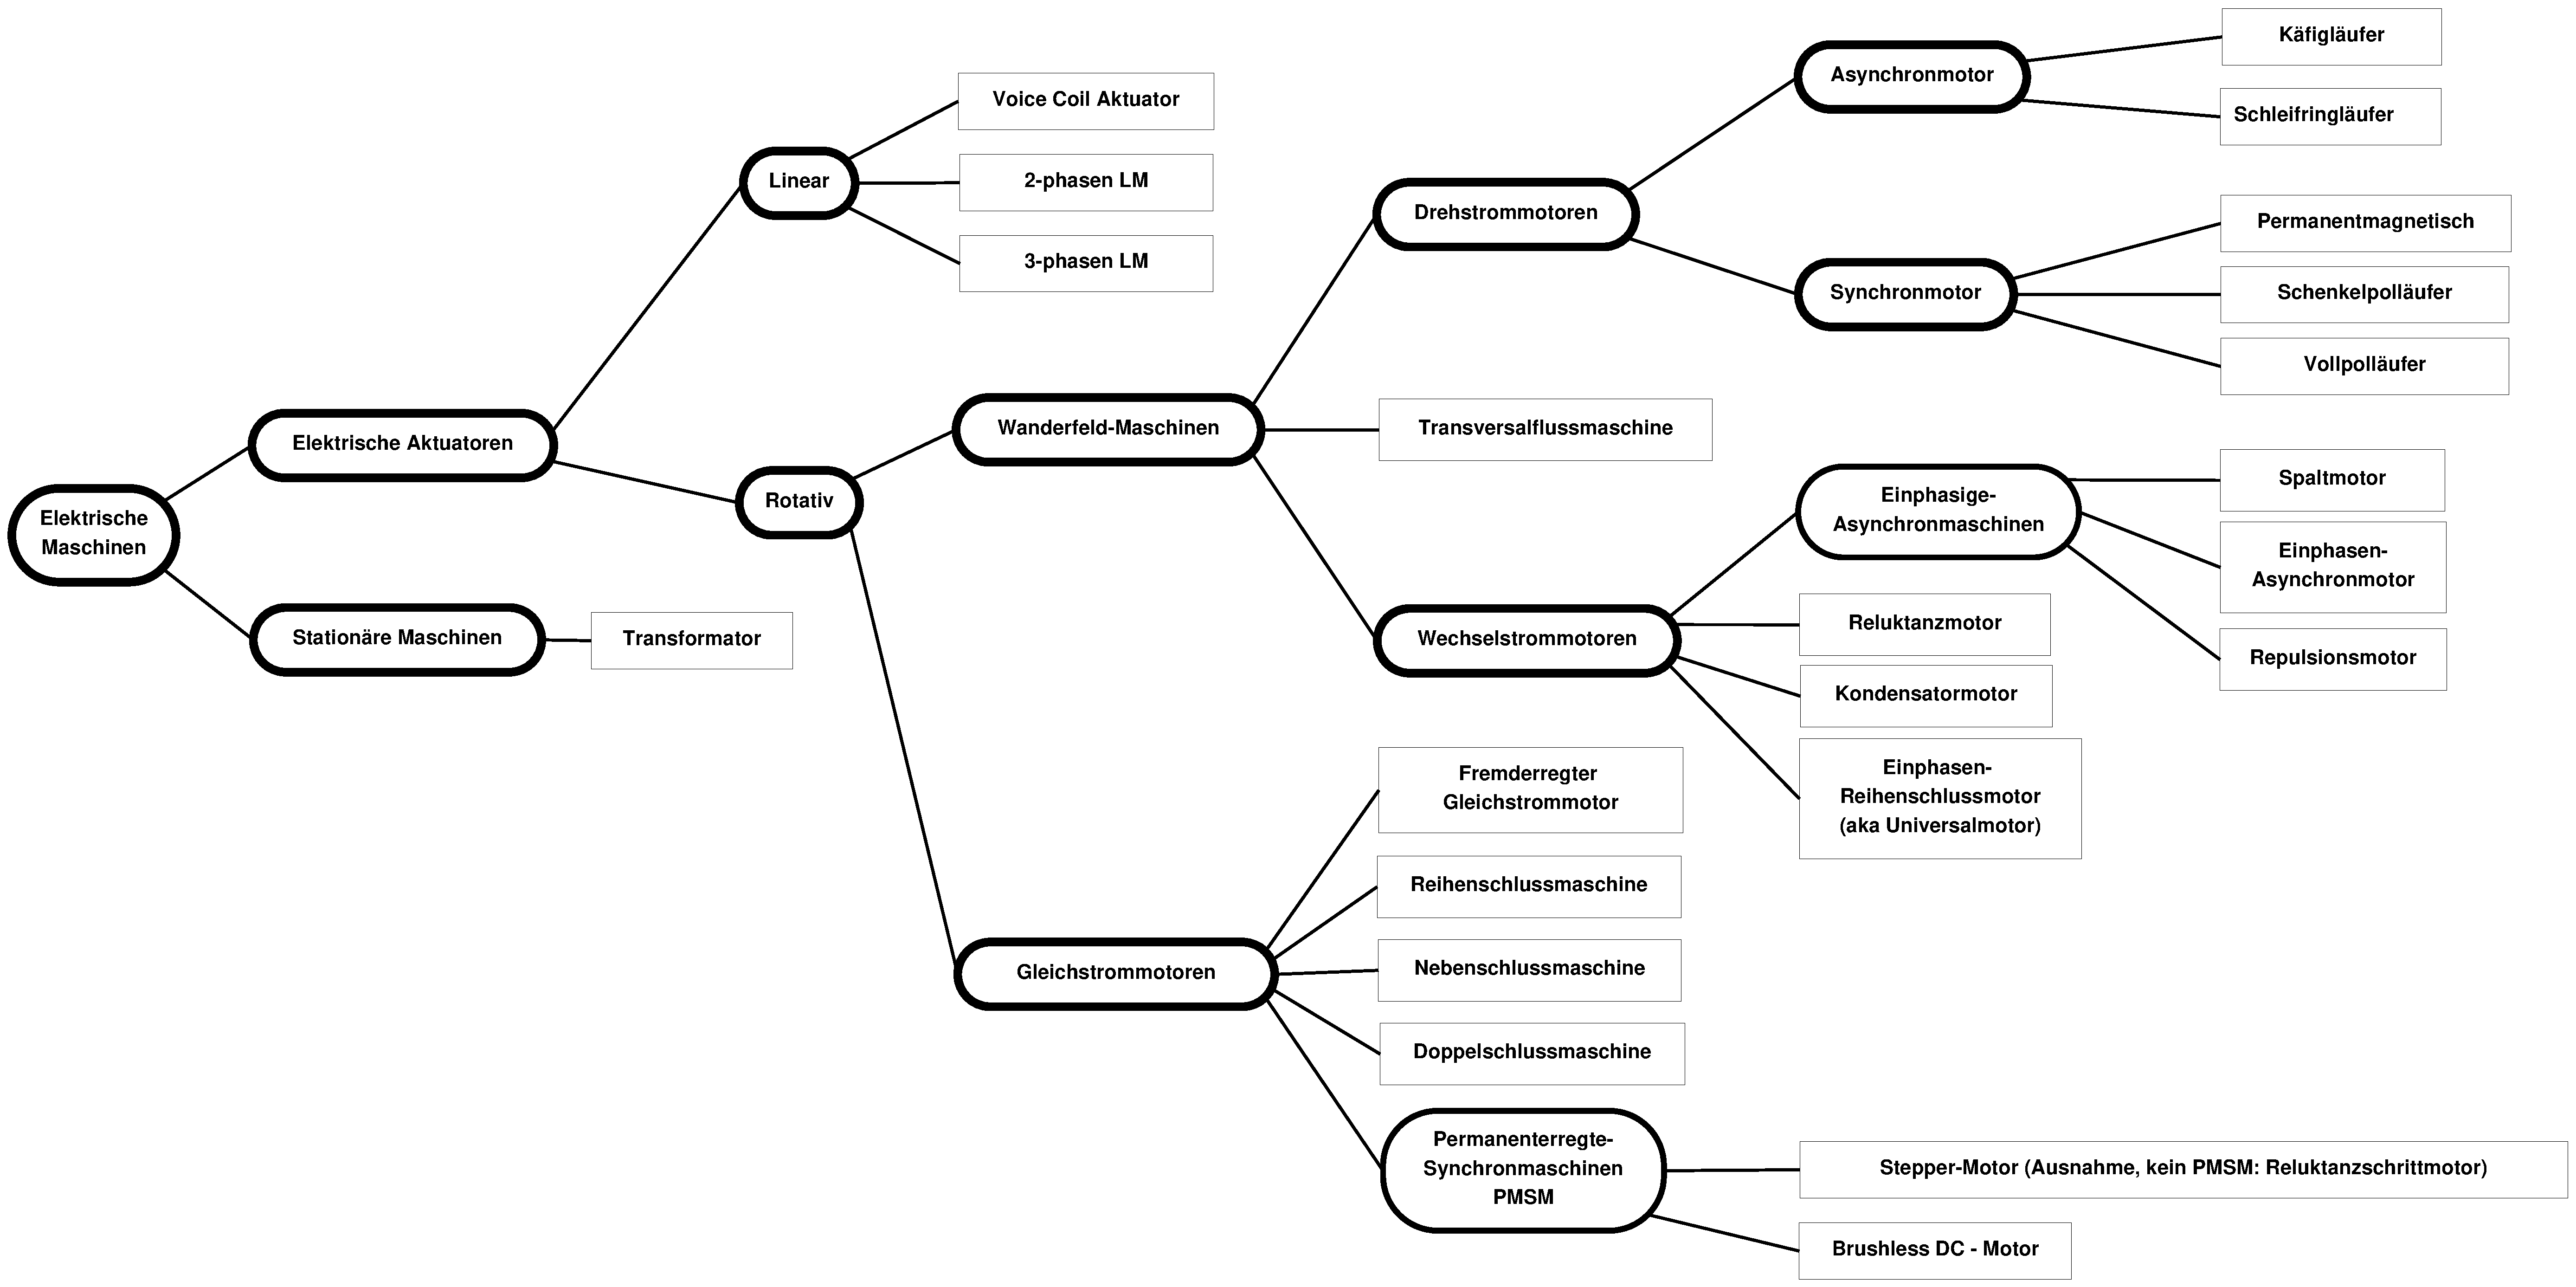
\includegraphics[width=1\linewidth]{./pics/elMasch}
		\end{figure}
		\subsection{Stationäre Maschinen}
		\subsubsection{Transformator}
		\subsection{Elektrische Aktuatoren}
			\leavevmode\\
			\textbf{\large Unterschiede zwischen Eisenlose und eisenbehaftete Motoren\\\\}
			Bei eisenlosen Motoren werden die Wicklungen mit Epoxid vergossen (Luftspaltwicklung). Diese Motoren sind für sehr gleichförmige Bewegungen geeignet. Bei ihnen wird keine magnetische Anziehungskraft erzeugt.
			Bei eisenbehafteten Motoren hingegen werden die Wicklungen in einem Eisenkäfig fixiert. Eisenbehaftete Motoren nutzen das Eisen, um den magnetischen Fluss zu bündeln und können so eine sehr hohe Kraftdichte erzeugen.\\\\			
			\textbf{Vorteile eisenlose Motoren:}
			\begin{itemize}
				\item Keine Eisenverluste (Eisenmagnet muss nicht umgepolt werden, die Hysteresekurve muss nicht durchlaufen werden, was Energie kostet)
				\item Kompakter und leichterer Forcer/Rotor
				\item Kleine Rotor Induktivität (weniger Elektromagnetische Störungen, schnelle Reaktionszeit des Stroms)
				\item Bei Sinuskommutierung erhält man ein gleichförmiges Moment bzw. eine konstant wirkende Kraft
			\end{itemize}
			\leavevmode \\
			\textbf{Vorteile eisenbehaftete Motoren:}
			\begin{itemize}
				\item sehr hohe Drehmomentdichte
				\item Maximierung der magnetischen Kraft
				\item höhere Spitzenkraft als eisenlose Motoren der selben Baugröße ($ \rightarrow $ kompaktere Ausführungen möglich)
			\end{itemize}
			
			\newpage	
			\subsubsection{Linearaktuatoren}				
				\begin{description}[leftmargin=2.5cm]
					\item[Allgemein]					
					Grundsätzlich arbeiten Linearmotoren wie rotatorische Motoren. Man kann sie sich so vorstellen, dass man einen beliebigen Motor aufschneidet und in die Ebene abwickelt.
					\leavevmode \\
					\begin{figure}[h!]
						\centering \rule{1.5cm}{0cm}
						\includegraphics[width=0.2\linewidth]{./pics/rot2lin} 
					\end{figure} 
					Wobei die ursprünglich kreisförmig angeordneten elektrischen Erregerwicklungen (Stator) auf einer ebenen Strecke angeordnet sind. Der Läufer, der im Drehstrommotor rotiert, wird beim Linearmotor von dem längs bewegten Magnetfeld über die Fahrstrecke bewegt. Analog dazu funktionieren tubulare Linearmotoren ebenfalls wie ihre rotativen Verwandten, jedoch ist bei Linearmotoren der Untershied einer begrenzten Stator-Streke.
					\begin{figure}[h!]
						\centering 
						\includegraphics[width=0.08\linewidth]{./pics/symbolLinearmotor}
						\caption{Symbol für Linearmotoren}
					\end{figure} \leavevmode \\

					\item[Einteilung]
					\leavevmode \\
					\begin{figure}[h!]
						\centering
						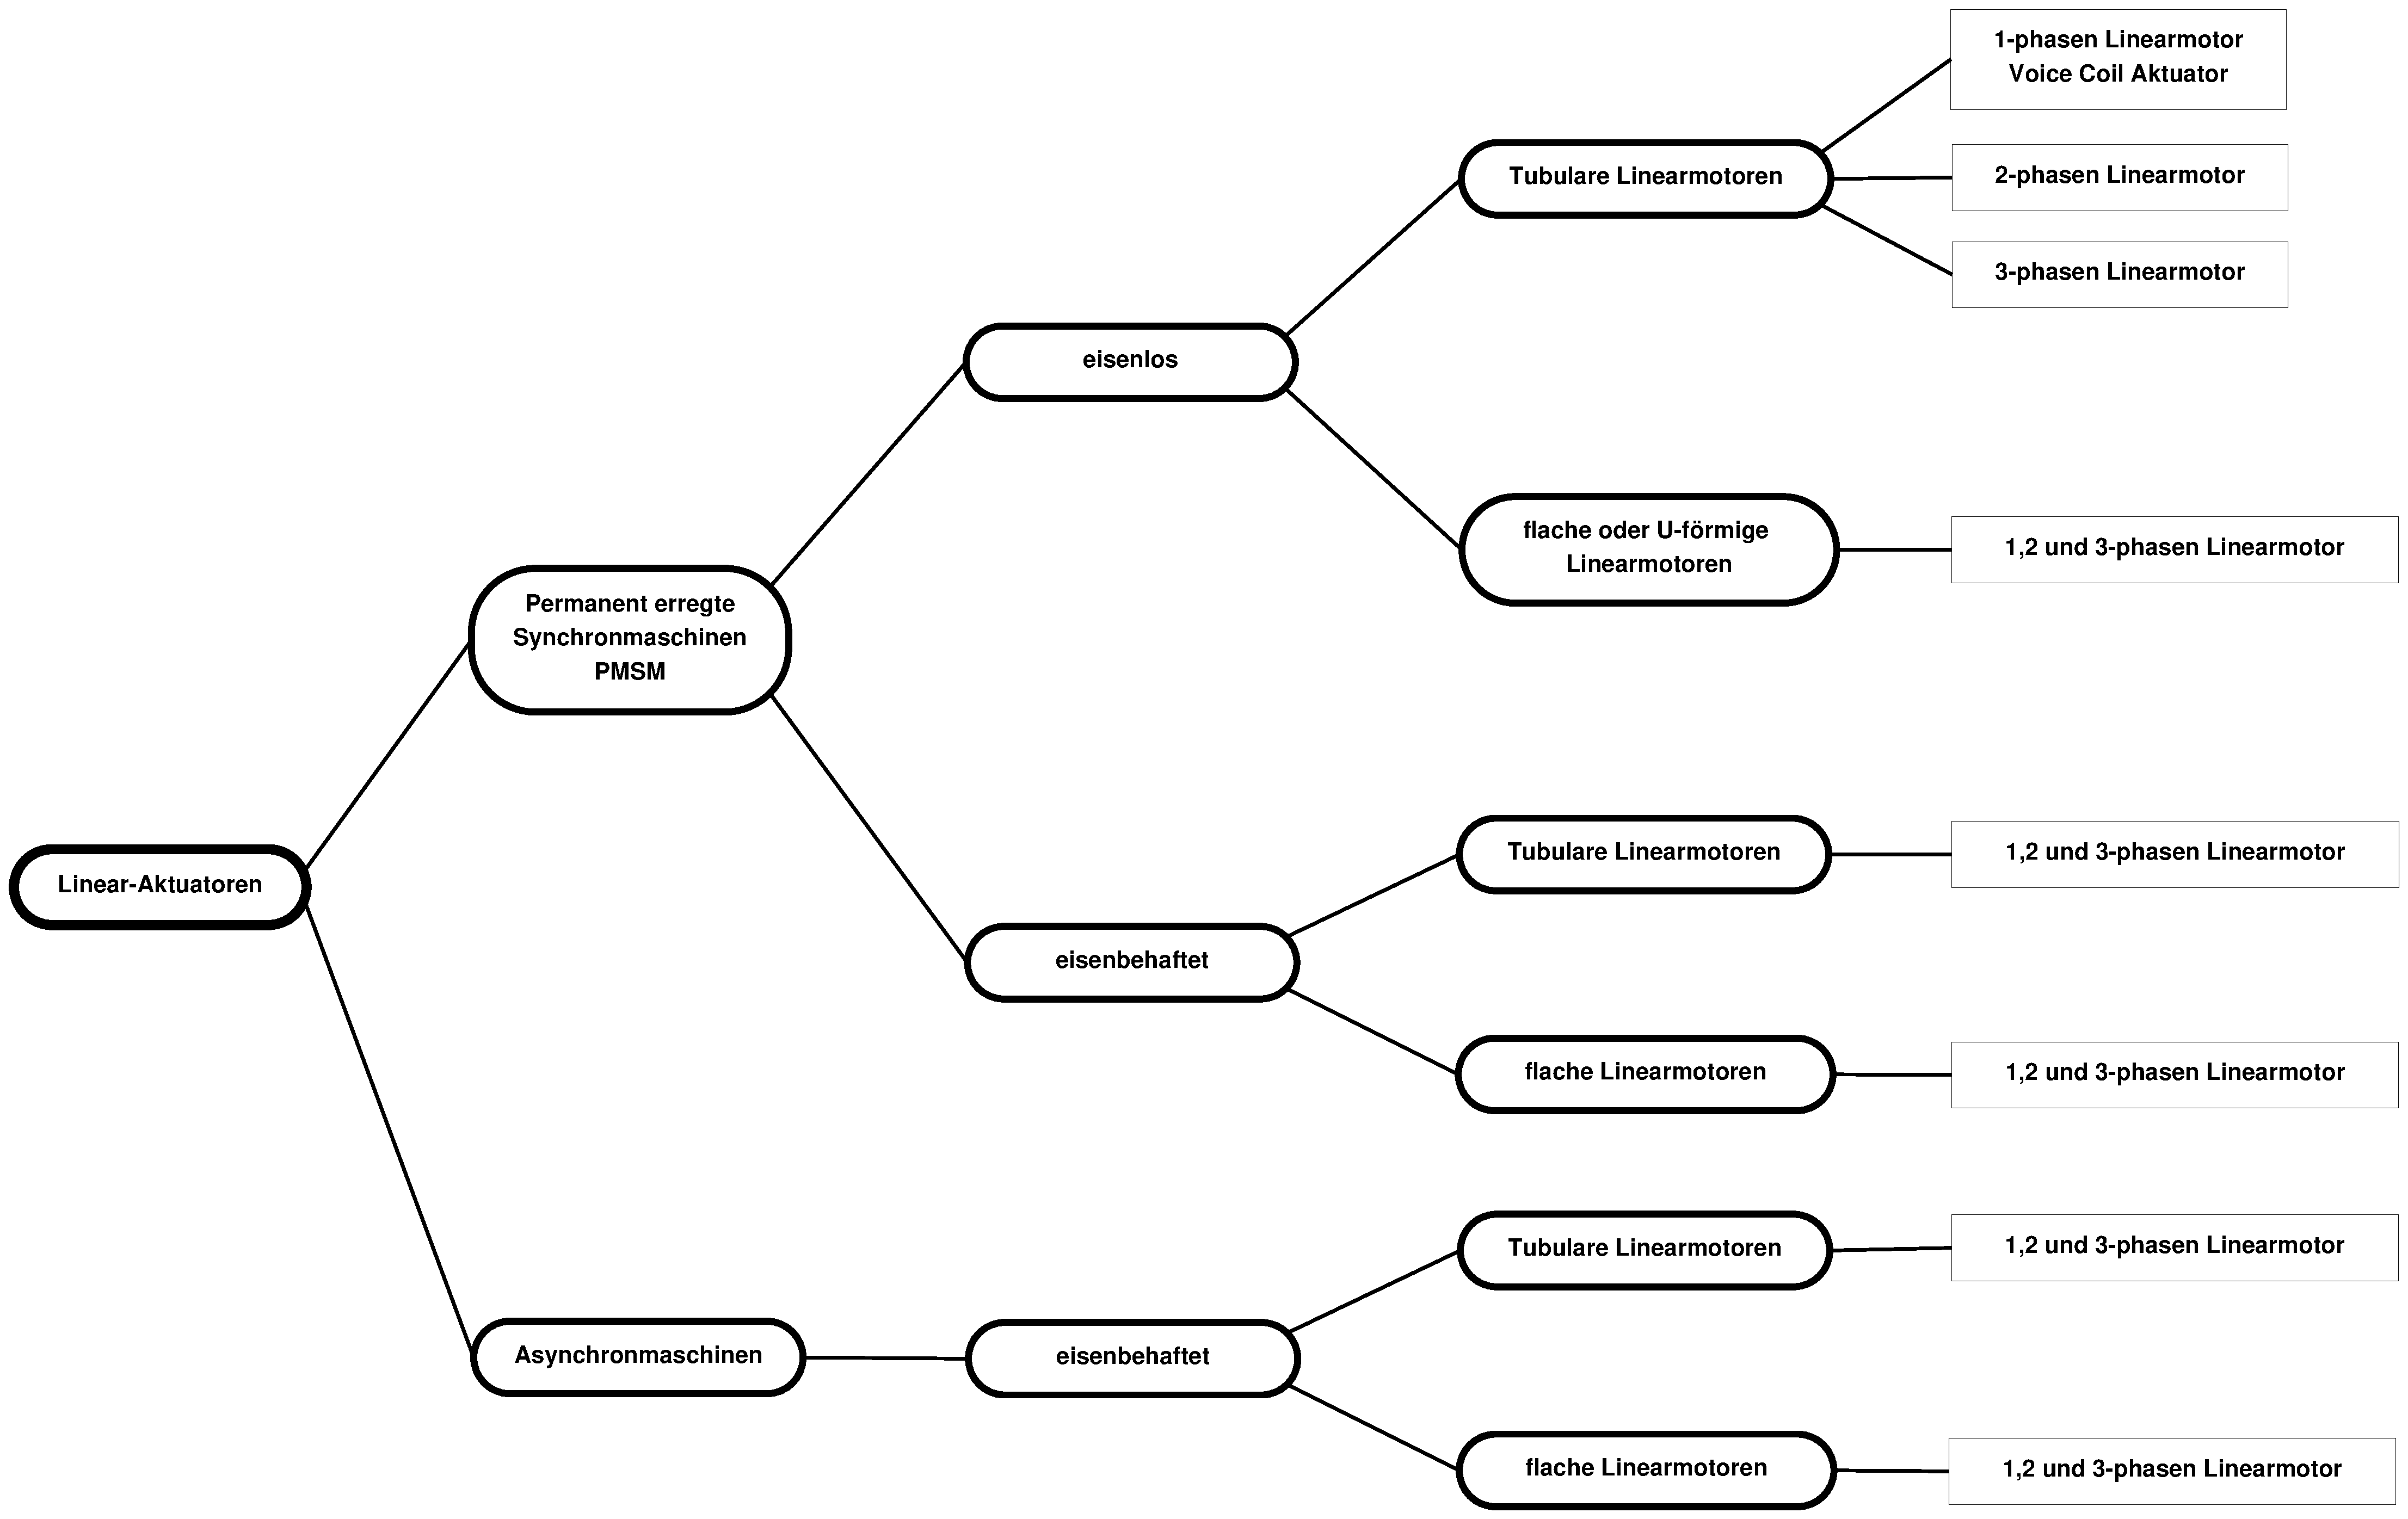
\includegraphics[width=0.9\linewidth]{./pics/LinearAktuatoren.eps}
					\end{figure}
				
					\item[Tubulare Linearmotoren] 
					Unter einem tubularen Linearmotor versteht man einen elektrischen Direktantrieb, bei dem die lineare Bewegung direkt aufgrund der elektromagnetischen Kraftwirkung erzeugt wird. Das heißt, die translatorische Bewegung wird nicht durch eine mechanische Umwandlung über eine Spindel, Riemen oder Kurvenscheibe erzeugt, sondern basiert direkt auf den Wechselwirkungen zwischen elektromagnetischen Kräften. Grundsätzlich können derartige Motoren sowohl nach dem Lorenzkraftprinzip wie auch nach dem Maxwellkraftprinzip (siehe Kap. \ref{reluktanzkraft}) aufgebaut werden und gehören zu der Gattung der Linearmotoren. Der Unterschied zu den flachen oder U-förmigen Linearmotoren besteht darin, dass die Erregerwicklung des Stators rohrförmig (tubular) und die Magnete des Läufers stabförmig sind. Konstruktiv gesehen entsteht so ein Antriebselement, das Ähnlichkeiten zu einem pneumatischen oder hydraulischen Zylinder aufweist. Im Bild ist ein permanenterregter Läufer abgebildet. Im asynchronen Fall besteht der Läufer statt aus Permanentmagneten, aus kurzgeschlossenen Kupferwindungen wie beim bekannten rotativen Asynchronmotor.
					\begin{figure}[!h]
						\centering \rule{1.5cm}{0cm}
						\includegraphics[width=0.55\linewidth]{./pics/tubular}
					\end{figure}
					
					\item[Flache, U-förmige Linearmotoren] 
					Bei flachen bzw. U-förmigen Linearmotoren befinden sich bei PMSM die Permanentmagneten am Stator des Motors. Beim asynchronen Linearmotor hält der Stator hingegen die Erregerwicklungen, die um weichmagnetisches Eisen gewickelt sind und somit Magnetfelder erzeugt.	Ein Linearmotor besteht aus nur zwei Komponenten: einem Wicklungspaket (Forcer bzw. Primärteil) und einem Träger (Magnetschiene bzw. Sekundärteil), auf dem die Permanentmagneten fixiert sind. Die Kupferwindungen des Wicklungspaketes sind entweder in Epoxidharz oder Eisen eingebettet. Die Kupferwindungen führen den gesamten Strom eines Linearmotors. 	
					\begin{figure}[h]
						\centering \rule{2.5cm}{0cm}
						\subfigure[U-förmiger Linearmotor]
						 {\includegraphics[width=0.4\textwidth]{./pics/LM}} \hspace{0.4cm}
						\subfigure[flacher Linearmotor] 
						 {\includegraphics[width=0.4\textwidth]{./pics/flatLM}}
					\end{figure}					
					Das Magnetassembly besteht aus Seltenen-Erde-Magneten, die in abwechselnder Polarität auf einem Stahlträger montiert sind. Sie erzeugen ein magnetisches Feld senkrecht zum Träger. Wenn in den Kupferwindungen Strom fließt, ergibt sich nach dem Lorentz´schen Gesetz eine Kraft $ F = I \times B $, die zur Beschleunigung der Masse benutzt wird. Eine Linearmotorachse besteht wiederum aus einem Linearmotor mit Lagerung und einem integrierten Positions-Gebersystem (Encoder). Der Forcer wird üblicherweise an den bewegten Teilen der Maschine befestigt. Das Magnetassembly wird am statischen Teil der Maschine fixiert. 
					\begin{figure}[h]
						\centering \rule{2.5cm}{0cm}
						\includegraphics[width=0.2\linewidth]{./pics/I.png} \hspace{1cm}
						\includegraphics[width=0.5\linewidth]{./pics/LM2} 
						\caption{Linke-Hand-Regel für die Wirkrichtung der Lorentzkraft}
						\label{}
					\end{figure}
					
					\item[Asynhroner Linearmotor] 
					Beim linearen Asynchronmotor wird die bewegende Kraft durch ein wanderndes Magnetfeld das mit einem Leiter interagiert, erzeugt. In jedem Leiter, sei es eine Windung, Spule oder einfach nur eine leitende Metallplatte, die im Feld platziert wird, werden Ströme induziert. Durch Wechselwirkung des magnetischen Wanderfeldes und dem induzierten Strom resultiert jene Kraft, die für eine Linearbewegung verantwortlich ist. Asynchrone Linearmotoren werden für Anwendungen die große Kräfte benötigen verwendet. Zum Beispiel elektrisch Schiebetüren oder Magnetschwebebahnen.
					
					\item[PSM als Linearmotor] 
					Die permanenterregte Synchronmaschine (PSM) als Linearmotor benötigt im Forcer einen sinusförmigen Stromverlauf um ohne rucken bewegt werden zu können. Dies kann entweder durch Einspeisung von Wechselstrom erreicht werden oder durch Sinuskommutierung einer Gleichspannung. 
					
					\item[Sinuskommutierung]										
					Ein hoher Gleichlauf kann erreicht werden, indem die Phasenströme graduell angeglichen werden. Der Linearmotor ist geometrisch so aufgebaut, dass sich die Back-EMF in Form einer Sinusspannung ergibt. Daher ist die beste Lösung einen sinusförmigen Stromverlauf vor zu gegeben, der dann zu einer gleichmäßigen Bewegung führt. Das erzeugte Drehmoment/ die erzeugte Kraft ist dann konstant. Einen sinusförmigen Strom nachzubilden verlangt aber eine höhere Positionsauflösung als von den Hallsensoren erhalten werden kann. Der Strom in den 3 Phasen muss viel häufiger angepasst werden. Darum verwendet die Sinuskommutierung meist Encoder zur präzisen Lagebestimmung des Rotors. Sinuskommutierung ermöglicht einen gleichmäßigen Motorbetrieb und ergibt sogar eine bessere Performance.						
				\end{description}
				
				\paragraph{1-phasen Linearmotor/ Linear Voice Coil Motor/ Tauchspulenaktuator}
					Der Voice Coil Aktor ist ein zweipoliger nichtkommutierter Antriebsmechanismus mit limitiertem Weg. Er besteht aus zwei Komponenten: einem Dauermagneten am fixierten Teil und einer Spule, die auf einen im Luftspalt beweglichen nichtmagnetischen Spulenkörper gewickelt ist. Im eingebauten Zustand befindet sich die Spule im Luftspalt des Magnetfeldes. Richtung und Amplitude der Lorentzkraft werden dabei von der Stromstärke und -richtung bestimmt. Sie arbeiten nach dem Lorentz-Kraft-Prinzip und sind dadurch bidirektional aktiv ansteuerbar. Die konstante Kraftverteilung über dem Hub ermöglicht eine hohe Startkraft, die verbunden mit der geringen Masse der bewegten Spule höchste Dynamik erlaubt. Zudem lässt sich eine extrem geringe Hysterese erreichen. Durch diese Eigenschaften empfehlen sich Tauchspulenaktuatoren vor allem für dynamische und präzise Regelungsanwendungen.
					\begin{figure}[h]
						\centering
						\includegraphics[width=0.6\linewidth]{./pics/vcm}
					\end{figure}
					\leavevmode \\
					
				\paragraph{2-phasen Linearmotor} 
					Das Funktionsprinzip ist das selbe wie im Kaptile Linearmotoren erklärt wird. In der Abbildung funktioniert der eisenbehaftete LM nach dem Reluktanzkraft-Prinzip (Kap. \ref{reluktanzkraft}).	\\
					\begin{figure}[h]
						\centering
						\includegraphics[width=0.6\linewidth]{./pics/2phase}
						\caption{2-phasiger, eisenbehafteter, U-förmiger Linearmotor}
					\end{figure} \\
					Die Magnetfelder des Läufers und die Magnetfelder des Stators (\glqq Fahrweg\grqq) werden immer so kombiniert (die Elektromagnete werden entsprechend gepolt mit Strom versorgt), dass der Läufer ein Wegstück „nach vorne“ gezogen wird (und vom Magnetfeld hinter sich abgestoßen wird). Hat er die Position erreicht, zu der er gezogen wurde, so wird umgepolt, und der Läufer wird von dieser Position nun weggedrückt und zur nächsten Magnetspule/Permanentmagnet hingezogen. Dadurch, dass der Läufer zwei etwas versetzte Magnetfeld-Erzeuger besitzt, befindet sich immer mindestens einer davon gerade „auf halbem Weg“, was eine Festlegung der Laufrichtung (vorwärts oder rückwärts) ermöglicht.
				\paragraph{\textcolor{red}{3-phasen Linearmotor}} 
			\subsubsection{\textcolor{red}{Rotationsaktuatoren}}
				\paragraph{Gleichstrommotoren} 
					\subparagraph{\textcolor{red}{Brushless DC-Motor}}
					\subparagraph{\textcolor{red}{Permanenterregte Synchronmaschine - PMSM}} 
					\subparagraph{\textcolor{red}{Steppermotor}}
					Anschluss, Eigenschaften, Vor- u Nachteile, Funktionsweise, Ansteuerung, Bauarten
					\subparagraph{Servomotor} 
					\textcolor{red}{Üblich gemeinter Motortyp wenn von Servomotor gesprochen wird - BrushlessDC, PMSM?}\\
					Als Servomotor werden Elektromotoren beliebiger Bauart (AC, DC) bezeichnet, die die Kontrolle der Winkelposition, Drehzahl und Winkelbeschleunigung ihrer Motorwelle erlauben. Sie bestehen aus einem Elektromotor, der zusätzlich mit einem Sensor (Encoder) zur Positionsbestimmung ausgestattet ist. Die vom Sensor ermittelte Winkelposition/ -geschwindigkeit der Motorwelle wird kontinuierlich an eine meist außerhalb des eigentlichen Motors angebrachte Regelelektronik übermittelt, den so genannten Servoregler, der die Bewegung des Motors entsprechend einem oder mehreren einstellbaren Sollwerten, wie etwa Soll-Winkelposition oder Solldrehzahl, regelt.
					\begin{figure}[h]
						\centering
						\includegraphics[width=0.5\linewidth]{./pics/servo}
						\caption{Die Kombination Servomotor und Servoregler wird als Servoantrieb bezeichnet}
	
					\end{figure}
					\leavevmode \\
					\subparagraph{Torque-Motor} 
					Torque-Motoren können als Außenläufer (Stator innen, Rotor außen) oder normale Innenläufer ausgeführt sein. Durch den verhältnismäßig großen Durchmesser, die hochpoligen Wicklungen können diese Motoren große Drehmomente bei geringen Drehzahlen erzeugen.
					\begin{itemize}
						\item[+] Große Beschleunigungen möglich $ \rightarrow $ hohe Dynamik des Systems
						\item[+] Antriebssteif $ \rightarrow $ kein Verdrehspiel $ \rightarrow $ geringere Störgrößen $ \rightarrow $ gute Regeleigenschaften
						\item[+] Kaum Verschleiß
						\item[-] Starke Wärmeentwicklung (muss oft Wassergekühlt werden)
						\item[-] Teuer
					\end{itemize}
					\begin{figure}[h]
						\centering
						\includegraphics[width=0.5\linewidth]{./pics/TM}
	
					\end{figure}
					\leavevmode \\
				\paragraph{Drehstrommotoren} 
					\subparagraph{\textcolor{red}{Synchronmotor}}
					\subparagraph{\textcolor{red}{Asynchronmotor}}
				\paragraph{Wechselstrommotoren} 